\input preamble_DPO.tex

\date{13 января 2021}		% Дата семинара
\setcounter{s}{1}			% Номер семинара

\begin{document}


\title{Дискретная математика:\\
множества и логика}

\institute{Факультет компьютерных наук, НИУ ВШЭ}

\begin{frame}
  \titlepage
\end{frame}


\begin{frame}{Математическое доказательство}

\acc{Утверждение} в математике --- то, что можно либо доказать, либо опровергнуть.
\spc

\acc{Доказательство} в математике --- цепочка логических умозаключений, показывающая, что при условии истинности не которого набора аксиом и правил вывода утверждение верно.
\spc

\acc{Аксиома} --- утверждение, которое принимается на веру без доказательства.


\exmpl $0.(9)=1.$

\end{frame}


\begin{frame}{Кванторы и обозначения}

\begin{itemize}

\item Квантор всеобщности --- $\forall.$

\item Квантор существования --- $\exists.$

\item Импликация (логическое следствие) --- $\Longrightarrow.$

\item Равносильность --- $\Longleftrightarrow.$

\end{itemize}

\exmpl $\forall$ натурального $n$ число $n^2+n+41$ является простым.

\exmpl $\exists$ положительные целые $x,\ y,\ z$ такие, что $313(x^3+y^3)=z^3.$

\exmpl $\forall$ натурального $n$ выполнено $$1+2+3+\dots +n=\frac{n(n+1)}{2}.$$

\exmpl \hspace{-2 pt}* $\forall$ натурального $n$ выполнено $$1^3+2^3+3^3+\dots +n^3=(1+2+3+\dots +n)^2.$$

\end{frame}

\begin{frame}{Математическая индукция}

\acc{Математическая индукция} --- способ доказательства утверждения, зависящего от натурального параметра.

\acc{Описание метода:}

Предположим, что требуется доказать каждое из утверждений $ P_{0},P_{2},\ldots ,P_{n},P_{n+1},\ldots $

Допустим, что
\begin{itemize}
\item {\bf (База индукции)} Установлено, что $P_0$ верно.

\item {\bf (Шаг индукции)} Для любого $n$ доказано, что если верно $P_{n}$, то верно $P_{n+1}$.
\end{itemize}

Тогда все утверждения верны.

\exmpl $\forall$ натурального $n$ выполнено равенство $$1+3+5+\dots +(2n-1)=n^2.$$

\end{frame}


\begin{frame}{Язык теории множеств}

\acc{Множество} --- совокупность элементов. Порядок элементов не важен. Элементы входят без повторений.

\exmpl Множество цифр $\{0,1,2,3,4,5,6,7,8,9\}.$

\exmpl Множество натуральных чисел $\NN =\{0,1,2,3,\dots \},$ множество целых чисел $\ZZ =\{0,1,-1,2,-2,\dots \}.$

Обозначения:

\begin{itemize}

\item $a \in A$ --- принадлежность элемента $a$ множеству $A$;

\item $A\subseteq B$ --- множество $A$ является подмножеством $B$ (любой элемент множества $A$ также является элементом множества $B$);

\item $A=B$ --- множества состоят из одинаковых наборов элементов;

\item $\varnothing$ --- пустое множество.

\end{itemize}

\end{frame}


\begin{frame}{Задание множества и операции}

\acc{Способы задания множества:}

\begin{itemize}

\item Перечисление $M=\{1,2,3,4\}$;

\item Описание условия $N=\{ x \ |\ x=2y+1, \ y\in \ZZ\}$.

\end{itemize}

\acc{Операции с множествами:}

\begin{itemize}

\item  \acc{объединение} $A \cup B$ состоит из элементов, которые
принадлежат хотя бы одному из множеств;

\item \acc{пересечение} $A \cap B$ состоит из элементов, которые принадлежат обоим множествам;

\item \acc{разность} $A \setminus B$ состоит из элементов, которые принадлежат $A$, но
не принадлежат $B$;

\item \acc{симметрическая разность} $A\vartriangle B$ состоит из элементов, принадлежащих ровно одному из множеств.

\end{itemize}

\end{frame}


\begin{frame}{Диаграммы Эйлера-Венна}

\centerline{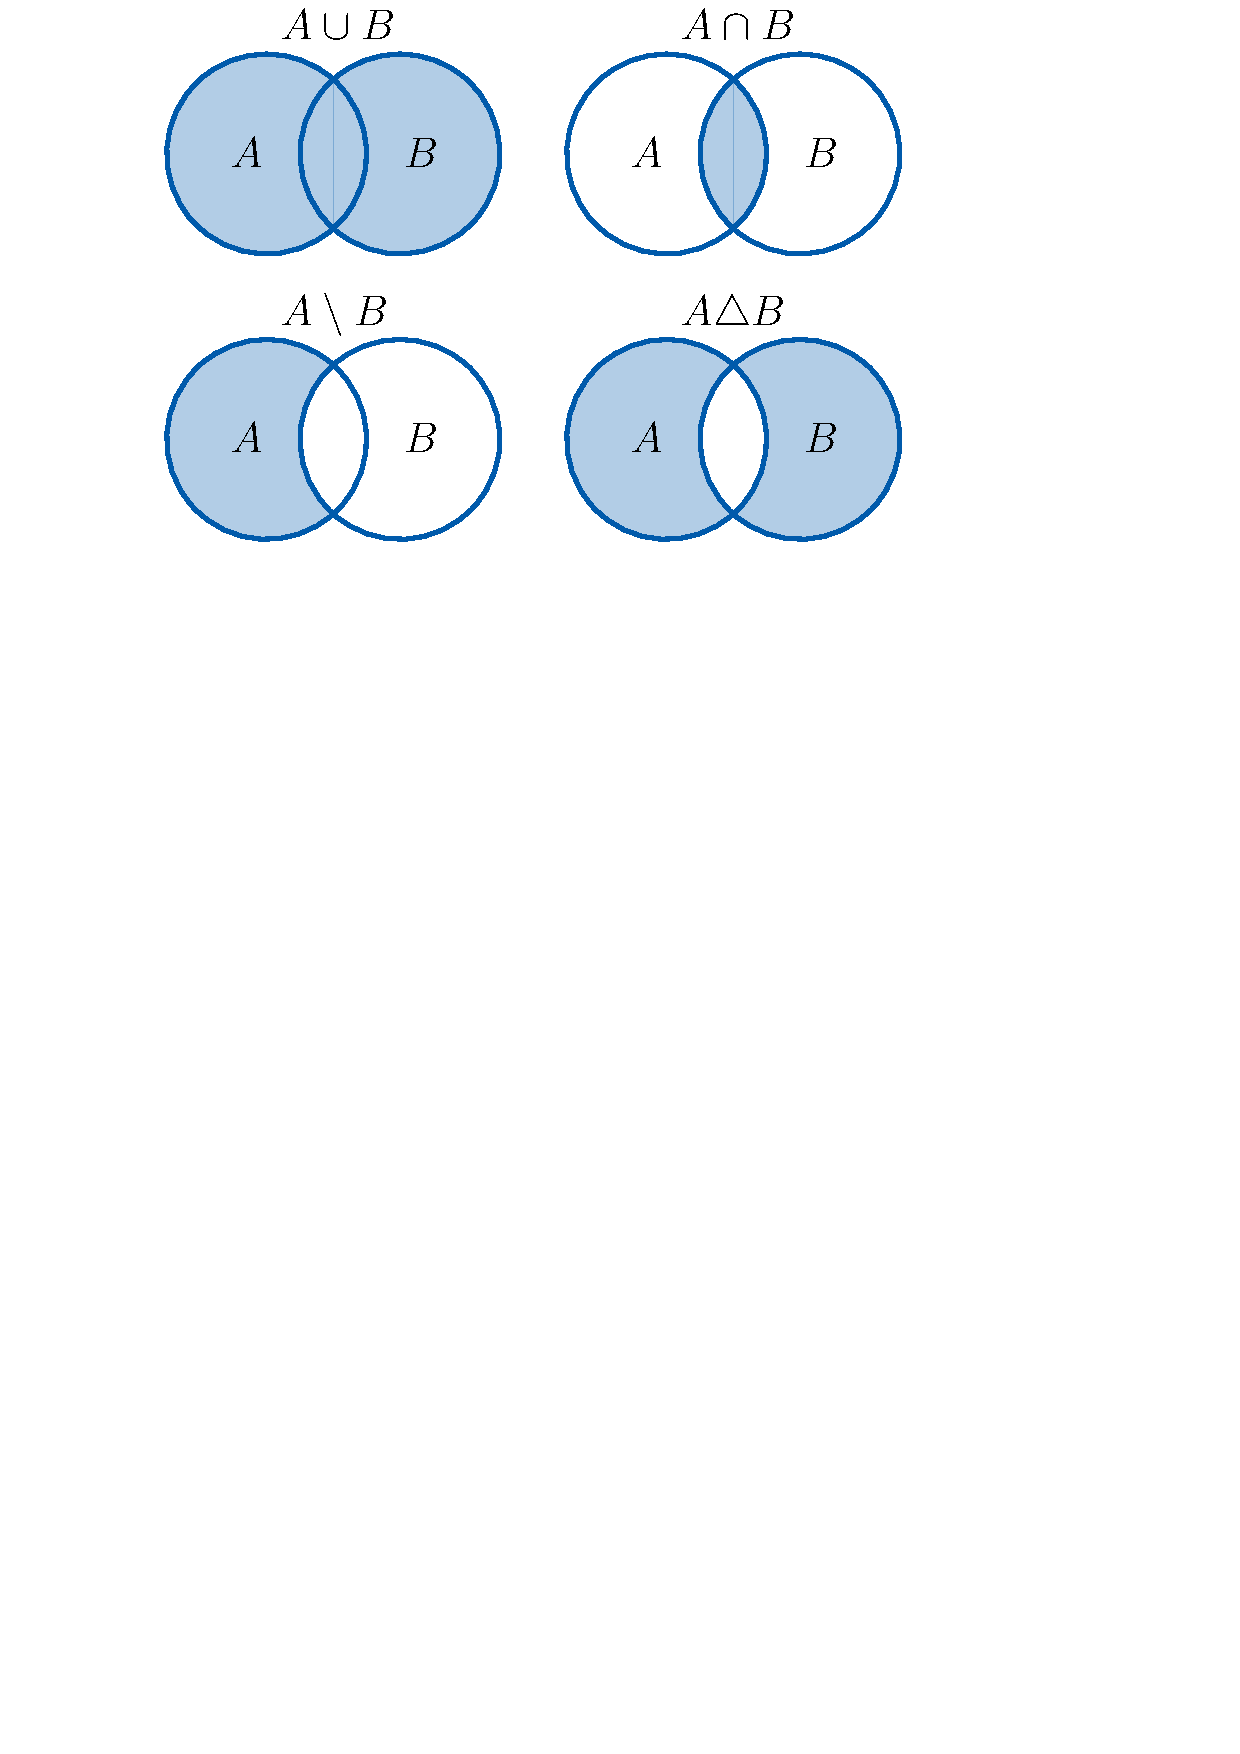
\includegraphics[scale=0.8]{img/venn-diagr.pdf}}

\end{frame}

\begin{frame}{Диаграммы Эйлера-Венна}

\exmpl Убедимся, что

{\bf a)} $A\subseteq B$ и $B\subseteq A \iff A=B;$

{\bf б)} $(A\setminus B) \cup (A\cap B)=A;$

{\bf в)} $(B\setminus A) \cup (A\setminus B)=A\triangle B.$

\end{frame}

\begin{frame}{Высказывания и предикаты}

\acc{Высказывание} --- утверждение, являющееся либо истиной, либо ложью.

\spc
\acc{Предикат} --- предложение, истинность которого можно проверить, подставив в него значения переменных.

\exmpl $a(x)=$ <<число $x$ больше $5$>> --- предикат. 

$c=$<<любую карту можно покрасить в четыре цвета так, чтобы соседние участки были различных цветов>> --- высказывание.

\spc

\exmpl <<Данное высказывание ложно>>.

Истинно ли это высказывание или нет?

\end{frame}

\begin{frame}{Логические операции с высказываниями}


С высказываниями и предикатами можно совершать операции:
\spc

\begin{tabular}{|c|c|c|}
\hline \bf Обозначение & \bf Значение & \bf Название  \\
\hline $a \wedge b$ & <<$a$ и $b$>> & конъюнкция  \\
\hline $a \vee b$ & <<$a$ или $b$>> & дизъюнкция \\
\hline $a \rightarrow b$ & <<из $a$ следует $b$>> & импликация \\
\hline $\neg a$ & <<не $a$>> & отрицание \\
\hline $a \equiv b$ ($a \leftrightarrow b$)& <<$a$ равносильно $b$>> & эквивалентность\\
\hline $a \oplus b$ & <<либо $a$, либо $b$>> & исключающее
ИЛИ\\
\hline
\end{tabular}

\exmpl Верно ли, что все живые сейчас тиранозавры умеют вышивать крестиком?

\exmpl Для целых чисел <<$x$ больше $5$>> $\wedge$ <<$x$ меньше $7$>> эквивалентно <<$x=6$>>.


\end{frame}

\begin{frame}{Таблица истинности}


Будем полагать $a=1$, если высказывание $a$ истинно, и $a=0$ в противном случае.
\spc
Как определены логические операции?
\spc
\begin{tabular}{|c|c|c|c|c|c|c|}
\hline$a$ & $b$ & $a \wedge b$ & $a \vee b$ & $a \rightarrow b$ & $a \equiv b$ & $a \oplus b$ \\
\hline 0 & 0 & 0 & 0 & 1 & 1 & 0 \\
\hline 0 & 1 & 0 & 1 & 1 & 0 & 1 \\
\hline 1 & 0 & 0 & 1 & 0 & 0 & 1 \\
\hline 1 & 1 & 1 & 1 & 1 & 1 & 0 \\
\hline
\end{tabular}

\end{frame}

\begin{frame}{Таблица истинности}


\exmpl Докажем следующие законы:

{\bf 1)} $1 \wedge a=a ; \quad$ {\bf 2)} $0 \wedge a=0 ; \quad$ {\bf 3)} $0 \vee a=a; \quad$
{\bf 4)} $1 \vee a=1$\\
{\bf 5)} $ \neg(\neg a)=a ; \quad $ {\bf 6)}$ \neg(a \wedge b)=\neg a \vee \neg b ; \quad$ {\bf 7)} $ \neg(a \vee b)=\neg a \wedge \neg b$\\
{\bf 8)} $a \wedge(b \vee c)=(a \wedge b) \vee(a \wedge c) ; \quad$ {\bf 9)} $a \vee(b \wedge c)=(a \vee b) \wedge(a \vee c)$

\end{frame}

\begin{frame}{Связь между языками логики и множеств}

Пусть $a(x)$ --- предикат <<число $x$ больше $5$>>, $b(x)$ --- <<число $x$ меньше $7$>>. Пусть $A= \{ x\ |\ x>5\},\ B= \{ x\ |\ x<7\}.$ Тогда предикат <<$x \in A$>> эквивалентен предикату $a(x)$, а <<$x \in B$>> эквивалентен $b(x)$.

Более того, предикат <<$x \in A\cup B$>> эквивалентен $a(x)\vee b(x)$, а <<$x \in A\cap B$>> эквивалентно $a(x)\wedge b(x)$.

\exmpl Выразим с помощью предикатов $a(x)$ и $b(x)$ и логических
связок предикат <<$x \in A\setminus B$>>.

\exmpl Докажем равенство $B\setminus (A \setminus B)=B.$

\end{frame}

\begin{frame}{Семинарская часть}

\z Пусть в некой деревне живёт брадобрей, который бреет всех жителей деревни, которые не бреются сами, и только их.

Бреет ли брадобрей сам себя?

\zh Докажите, что $\forall$ натурального $n$ выполнено $$1^3+2^3+3^3+\dots +n^3=(1+2+3+\dots +n)^2.$$

\z Докажем, что все лошади в мире одного цвета.

\z $x,y,z$ – целые числа, для которых истинен предикат
$$\neg(x=y) \wedge((y<x) \rightarrow(2 z>x)) \wedge((x<y) \rightarrow(x>2 z))$$
Чему равно $x$, если $z = 7,\ y = 16$?

\end{frame}

\begin{frame}{Семинарская часть}


\z Для какого слова {\it ложно} высказывание
<<Первая буква слова гласная $\rightarrow$ (Вторая буква слова гласная $\vee$ Последняя буква слова гласная)>>?

{\bf 1)} Жара \quad {\bf 2)} Орда \quad {\bf 3)} Огород \quad {\bf 4)} Парад

\z  Докажите, что $a \rightarrow b=\neg a \vee b$

\z Докажите, что для любых множеств $A,\ B,\ C$ выполняются равенства


\p $A \setminus (A \setminus  B)=A \cap B;$\quad
\p $B \cup(A \setminus  B)=A \cup B ;$

\p $(A \cup B) \setminus (A \cap B)=(A \setminus  B) \cup(B \setminus  A);$

\p $(A \cup B) \setminus  C=(A \setminus  C) \cup(B \setminus  C)$.

\end{frame}


\end{document}


